%!TEX root = ../main.tex



\section{Εισαγωγή}

\lettrine[findent=2pt]{\fbox{\textbf{Σ}}}{ε} αυτό το κεφάλαιο θα παρουσιαστούν τα πειράματα που έγιναν έτσι ώστε να υπάρχει εφαρμογή στην πράξη της θεωρίας και όσων έχουν αναφερθεί στα προηγούμενα κεφάλαια. Με αυτόν τον τρόπο μελετάται και κατά πόσο ο ελεγκτής που σχεδιάστηκε είναι ικανός να ελέγξει ικανοποιητικά διάφορα συστήματα ελέγχου. Σε κάθε ενότητα θα παρουσιάζεται ένα από τα διαθέσιμα συστήματα, το μαθηματικό μοντέλο του και τα αποτελέσματα του ελέγχου που παρέχει ο αυτο-ρυθμιζόμενος PID ελεγκτής. Τέλος, η κάθε ενότητα κλείνει με το σχολιασμό των πειραματικών αποτελεσμάτων.

\section{Σύστημα Mass-Springer-Damper}

\subsection{Μαθηματικό Μοντέλο}

Το πρώτο σύστημα που θα αναλυθεί είναι το σύστημα Μάζα-Ελατήριο-Αποσβεστήρας (Σχήμα \ref{fig:mass_spring_damper}) που αποτελεί ένα από τα πιο κλασικά συστήματα ελέγχου καθώς οι δυναμικές σχέσεις που το διέπουν δεν είναι περίπλοκες και είναι εύκολη η κατανόηση τους.

\begin{figure}[h]
  \centering
  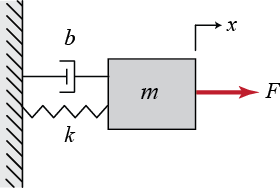
\includegraphics[width=\textwidth,height=5cm,keepaspectratio]{mass_spring_damper}
  \caption{Μοντέλο συστήματος Μάζας-Ελατηρίου-Αποσβεστήρα}
  \label{fig:mass_spring_damper}
\end{figure}

\noindent
H διαφορική εξίσωση που χαρακτηρίζει το σύστημα αυτό είναι
\begin{equation}
m\ddot{x} + b\dot{x} + kx = F
\label{eq:mass_springer_damper_ode}
\end{equation}
όπου $m$ είναι η μάζα, $x$ είναι η μετατόπιση της μάζας από το σημείο ισορροπίας, $b$ είναι η απόσβεση που παρέχει ο αποσβεστήρας, $k$ είναι η σταθερά του ελατηρίου και $F$ είναι η δύναμη που ασκείται στο σύστημα. Παίρνοντας το μετασχηματισμό Laplace της παραπάνω εξίσωσης έχουμε
\begin{equation}
ms^2X(s) + bsX(s) + kX(s) = F(s)
\label{eq:mass_springer_damper_laplace}
\end{equation}
Συνεπώς η συνάρτηση μεταφοράς (\emph{Transfer Function}) μεταξύ της εισόδου, που είναι η δύναμη $F(s)$, και της εξόδου, που είναι η μετατόπιση της μάζας $X(s)$, είναι
\begin{equation}
\frac{X(s)}{F(s)} = \frac{1}{ms^2 + bs + k}
\end{equation}

\subsection{Πείραμα}

Έστω ότι $\displaystyle m = 1\ kg$, $\displaystyle b = 10\ \frac{Ns}{m}$, $\displaystyle k = 20\ \frac{N}{m}$, $\displaystyle F = 1\ N$. Αντικαθιστώντας αυτές τις τιμές στην εξίσωση \ref{eq:mass_springer_damper_laplace} έχουμε
\begin{equation}
\frac{X(s)}{F(s)} = \frac{1}{s^2 + 10s + 20}
\end{equation}

\subsubsection{Απόκριση Χωρίς Έλεγχο}

Στο Σχήμα \ref{fig:mass_springer_damper_no_control} φαίνεται η βηματική απόκριση του συστήματος όταν δεν υπάρχει έλεγχος. Καθίσταται εμφανές ότι από μόνο του το σύστημα έχει μη ικανοποιητική απόκριση καθώς η τελική τιμή της εξόδου του είναι $y(t) = 0,047619$ και έχει ποσοστό σφάλματος \textit{offset error}$= 95.238 \%$. Συνεπώς κρίνεται απαραίτητη η χρήση ελεγκτή. Τα κέρδη του θα υπολογιστούν χρησιμοποιώντας τη μέθοδο αυτο-ρύθμισης που έχει περιγραφεί.

\begin{figure}[h]
  \centering
  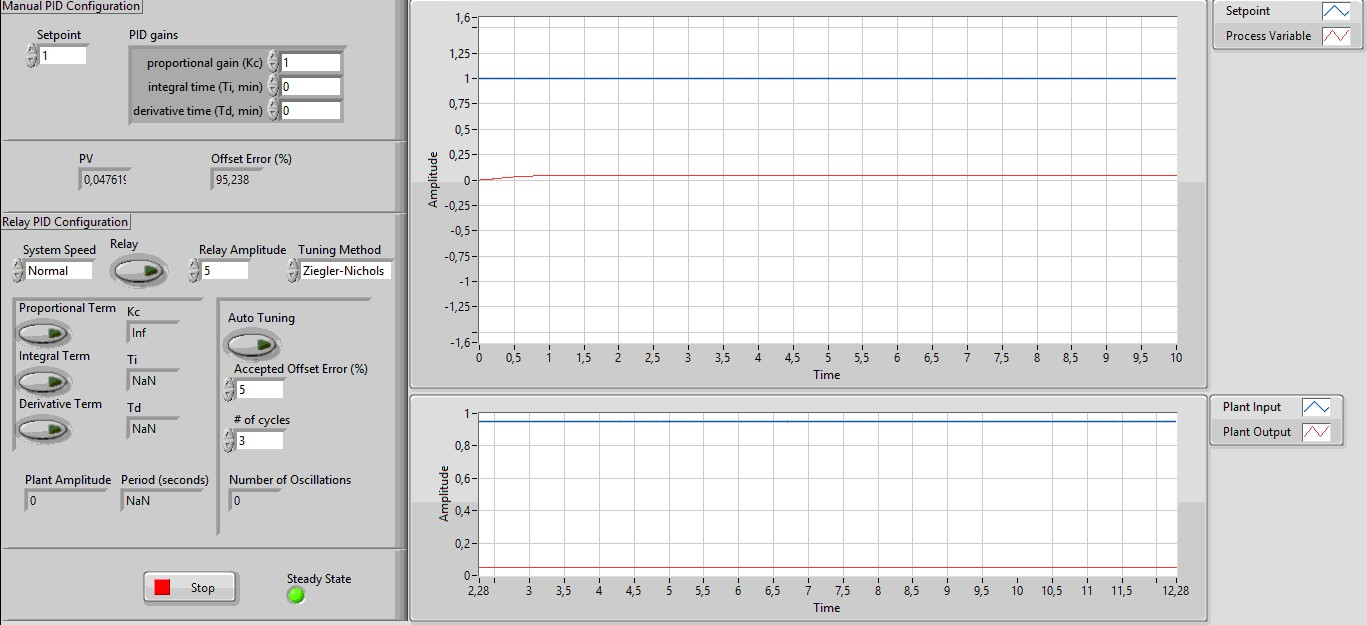
\includegraphics[width=\textwidth,height=5cm,keepaspectratio]{mass_springer_damper_no_control}
  \caption{Βηματική απόκριση του συστήματος Μάζα-Ελατήριο-Αποσβεστήρας χωρίς έλεγχο}
  \label{fig:mass_springer_damper_no_control}
\end{figure}

\subsubsection{Αναλογικός Έλεγχος}

Στο Σχήμα \ref{fig:mass_springer_damper_proportional_control} φαίνεται η βηματική απόκριση του συστήματος όταν σε αυτό εφαρμόζεται αναλογικός έλεγχος. Το κέρδος $K_c$ του αναλογικού όρου υπολογίστηκε αυτόματα, χρησιμοποιώντας τους τύπους από τη μέθοδο Ziegler-Nichols. Βλέπουμε ότι με τη χρήση του αναλογικού ελέγχου το σφάλμα βελτιώθηκε στο βαθμό η τελική τιμή του συστήματος να έχει πλέον μόνο $3,624\%$ απόκλιση από την επιθυμητή τιμή, αλλά, όπως είχε αναφερθεί και στην ενότητα \ref{subsec:proportional_control}, δεν μπορεί να το μηδενίσει. Επίσης, ο έλεγχος εισήγαγε ταλαντώσεις και υπέρβαση κατά ένα ποσοστό περίπου $50\%$. Αυτό, ανάλογα με τις απαιτήσεις ελέγχου, μπορεί να μην είναι αποδεκτό.

Στο ίδιο σχήμα φαίνεται η αριθμητική τιμή του πλάτους και της περιόδου των ταλαντώσεων που υπολόγισε ο αλγόριθμος. Το Σχήμα \ref{fig:mass_springer_damper_oscillations} αποτελεί μεγέθυνση του \ref{fig:mass_springer_damper_proportional_control} και αποδεικνύει ότι ο αλγόριθμος είναι πολύ ακριβής στην εύρεση των χαρακτηριστικών των ταλαντώσεων. 

\begin{figure}[h]
  \centering
  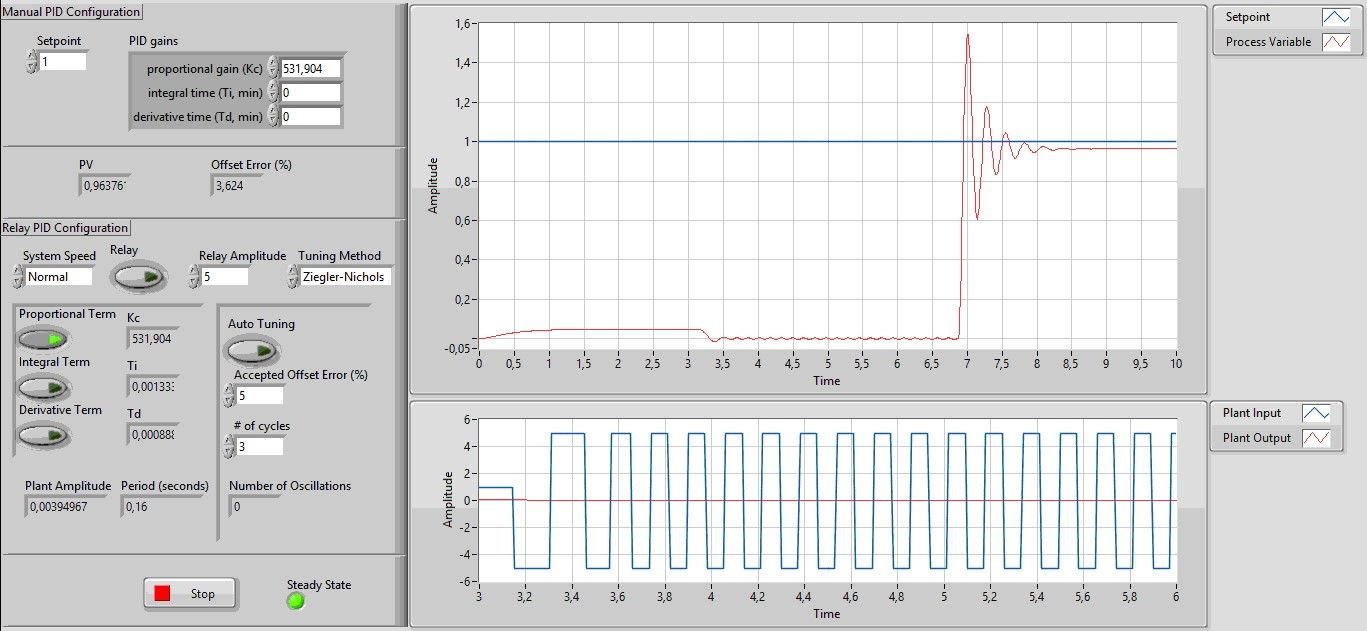
\includegraphics[width=\textwidth,height=5cm,keepaspectratio]{mass_springer_damper_proportional_control}
  \caption{Βηματική απόκριση του συστήματος Μάζα-Ελατήριο-Αποσβεστήρας με εφαρμογή αναλογικού ελέγχου}
  \label{fig:mass_springer_damper_proportional_control}
\end{figure}

\begin{figure}[h]
  \centering
  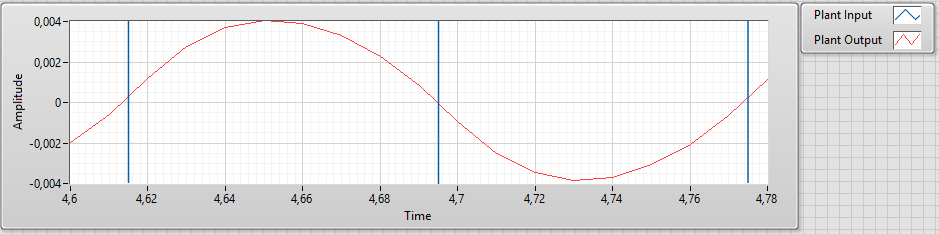
\includegraphics[width=\textwidth]{mass_springer_damper_oscillations}
  \caption{Μεγέθυνση των ταλαντώσεων του συστήματος κατά τη διάρκεια του πειράματος relay}
  \label{fig:mass_springer_damper_oscillations}
\end{figure}

\subsubsection{Αναλογικός-Ολοκληρωτικός Έλεγχος}

Το πείραμα επαναλαμβάνεται αλλά αυτή τη φορά χρησιμοποιείται και ο ολοκληρωτικός όρος προκειμένου να εξαλειφθεί το σφάλμα μόνιμης κατάστασης. Όπως φαίνεται από το Σχήμα \ref{fig:mass_springer_damper_integral_control}, η προσθήκη του ολοκληρωτικού όρου, όχι μόνο δεν μηδενίζει το σφάλμα μόνιμης κατάστασης αλλά χειροτερεύει την απόκριση του συστήματος σε σημείο να το οδηγεί να εκτελεί ταλαντώσεις γύρω από το επιθυμητό σημείο. Αυτό χωρίς αμφιβολία, είναι μία μη αποδεκτή κατάσταση.

\begin{figure}[h]
  \centering
  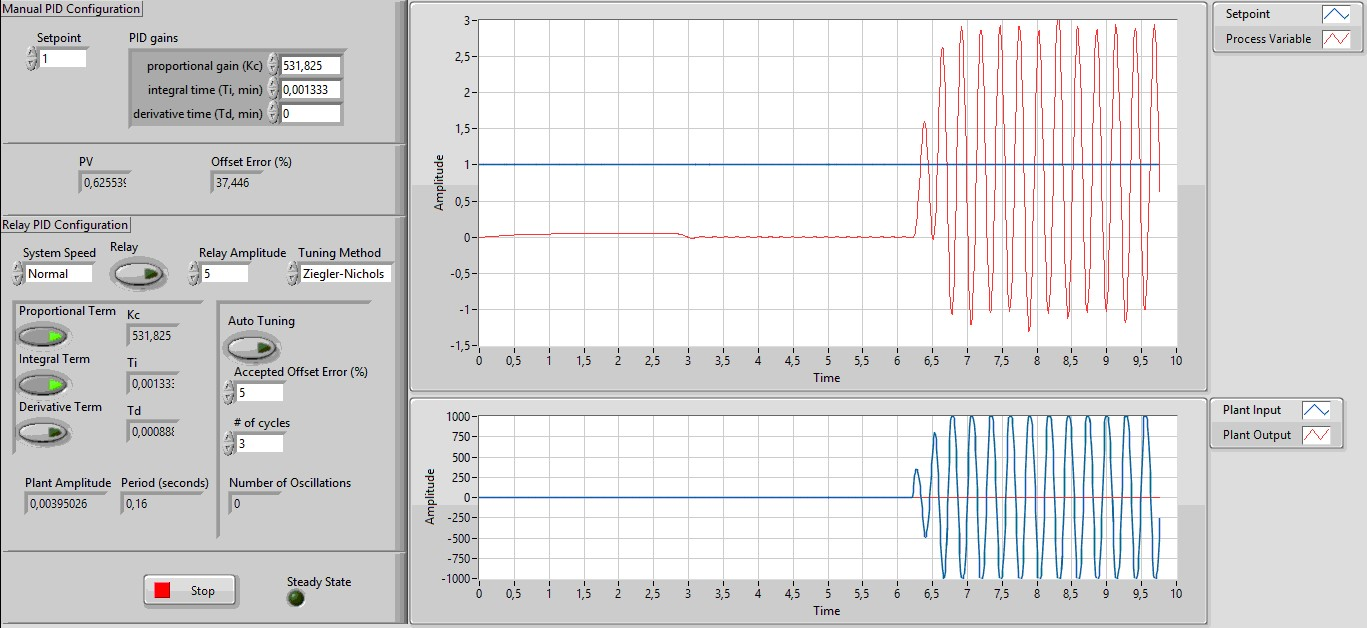
\includegraphics[width=\textwidth,height=5cm,keepaspectratio]{mass_springer_damper_integral_control}
  \caption{Βηματική απόκριση του συστήματος Μάζα-Ελατήριο-Αποσβεστήρας με εφαρμογή αναλογικού-ολοκληρωτικού ελέγχου}
  \label{fig:mass_springer_damper_integral_control}
\end{figure}

\subsubsection{Αναλογικός-Ολοκληρωτικός-Διαφορικός Έλεγχος}

Προκειμένου να βελτιωθεί η ευστάθεια του συστήματος εισάγεται και ο διαφορικός όρος. Ενώ ο ολοκληρωτικός όρος εισάγει έναν πόλο στο σύστημα, ο διαφορικός όρος εισάγει ένα μηδενικό βελτιώνοντας έτσι την ευστάθεια. Όπως φαίνεται στο Σχήμα \ref{fig:mass_springer_damper_derivative_control} η απόκριση βελτιώθηκε αισθητά. Ο έλεγχος που παρέχουν και οι τρεις όροι, όχι μόνο μηδένισε το σφάλμα μόνιμης κατάστασης όπως ήταν αναμενόμενο λόγω του ολοκληρωτικού όρου, αλλά βελτίωσε και τη μεταβατική κατάσταση του συστήματος. Η υπέρβαση, που πριν είχε ποσοστό σχεδόν $50\%$ τώρα έχει ποσοστό περίπου $20\%$. Επίσης έχει χρόνο ανύψωσης λιγότερο από ένα δευτερόλεπτο. Πλέον η απόκριση του συστήματος κρίνεται ικανοποιητική.

\begin{figure}[h]
  \centering
  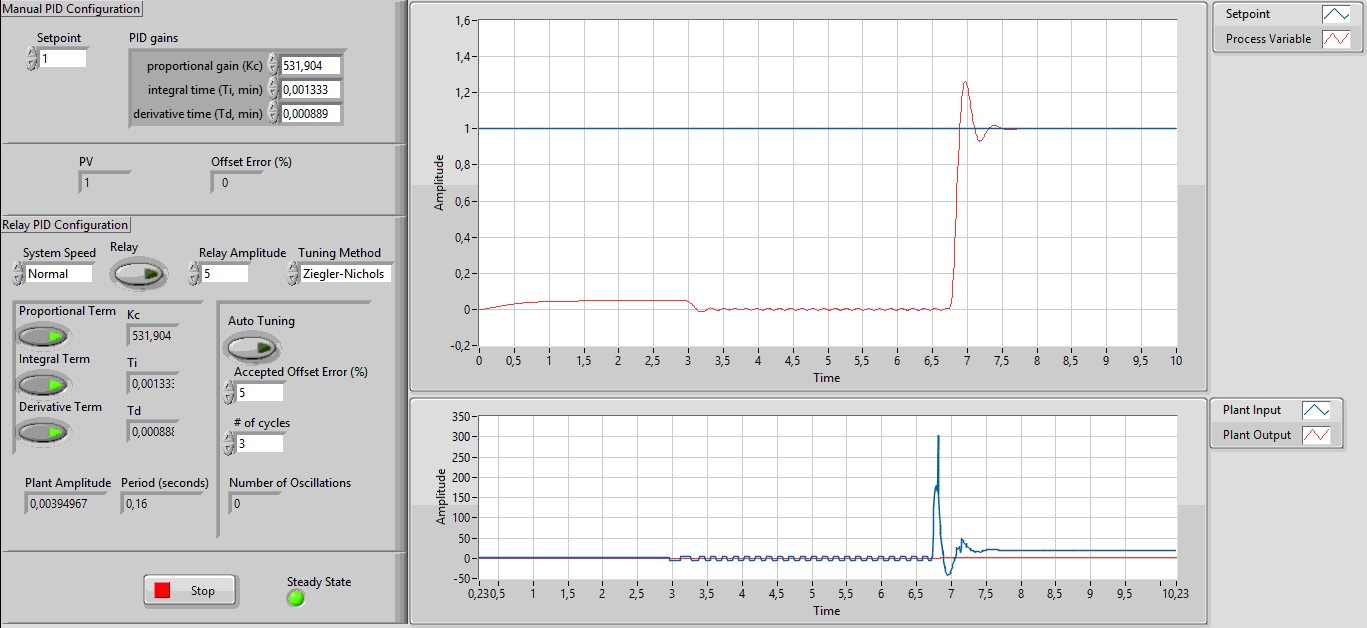
\includegraphics[width=\textwidth,height=5cm,keepaspectratio]{mass_springer_damper_derivative_control}
  \caption{Βηματική απόκριση του συστήματος Μάζα-Ελατήριο-Αποσβεστήρας με εφαρμογή αναλογικού-ολοκληρωτικού-διαφορικού ελέγχου}
  \label{fig:mass_springer_damper_derivative_control}
\end{figure}

Όπως έχει αναφερθεί κάθε διεργασία μπορεί να έχει διαφορετικές απαιτήσεις ελέγχου. Μπορεί για μία συγκεκριμένη εφαρμογή, η υπέρβαση που παρουσιάζει ο έλεγχος με αυτά τα κέρδη να μην είναι αποδεκτός. Έχει ενδιαφέρον λοιπόν να δούμε πώς ανταποκρίνεται το σύστημα σε διαφορετικές τιμές των κερδών. Ορίζοντας την επιθυμητή ταχύτητα του κλειστού συστήματος σε ``Slow" αντί για ``Normal" έχουμε την παρακάτω απόκριση. Από το διάγραμμα βλέπουμε ότι πλέον το σύστημα δεν παρουσιάζει υπέρβαση αλλά ως αντάλλαγμα αργεί αισθητά περισσότερο να φτάσει στην επιθυμητή τιμή.

\begin{figure}[h]
  \centering
  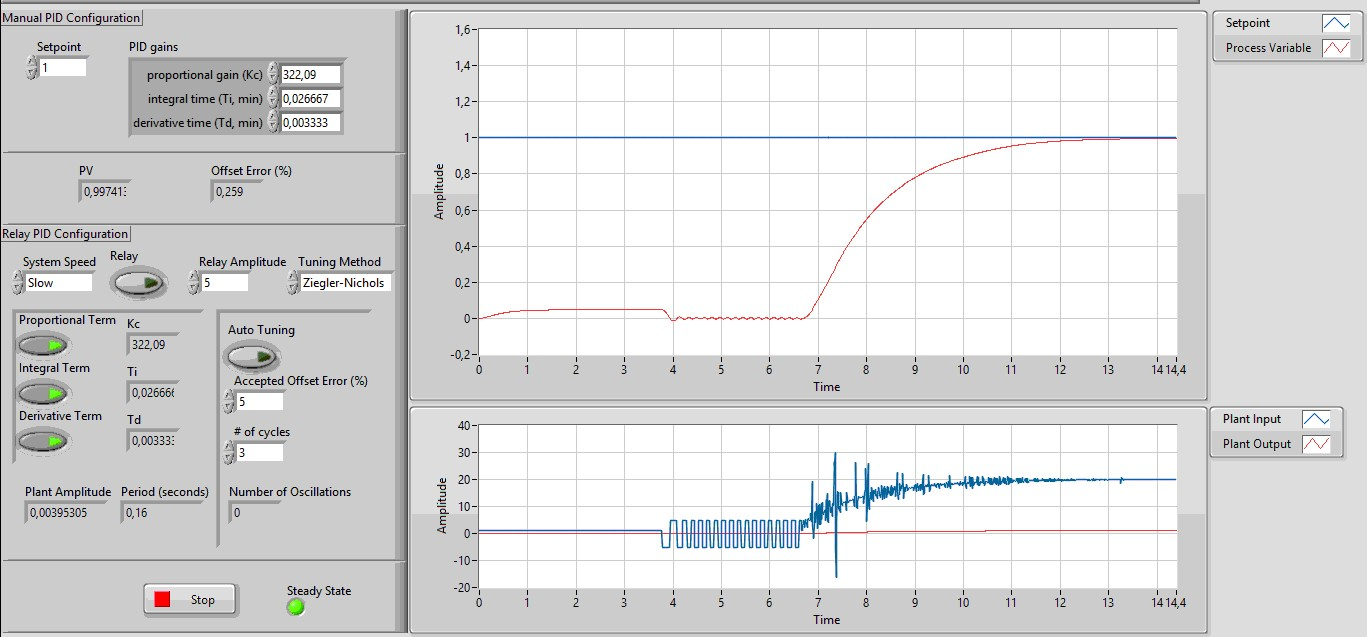
\includegraphics[width=\textwidth,height=5cm,keepaspectratio]{mass_springer_damper_ZN_slow}
  \caption{Βηματική απόκριση του συστήματος Μάζα-Ελατήριο-Αποσβεστήρας με εφαρμογή αναλογικού-ολοκληρωτικού-διαφορικού ελέγχου στη λειτουργία ``Slow"}
  \label{fig:mass_springer_damper_ZN_slow}
\end{figure}

Ακόμα, στο Σχήμα \ref{fig:mass_springer_damper_TL} φαίνεται η βηματική απόκριση του κλειστού συστήματος όταν τα κέρδη του ελεγκτή έχουν υπολογιστεί με τους τύπους Tyreus-Luyben. Η απόκριση μοιάζει σαν μια μίξη των δύο προηγούμενων αποκρίσεων. Η έξοδος του συστήματος δεν παρουσιάζει υπέρβαση, αλλά φτάνει και στην επιθυμητή τιμή μέσα σε περίπου ένα δευτερόλεπτο.

\begin{figure}[h]
  \centering
  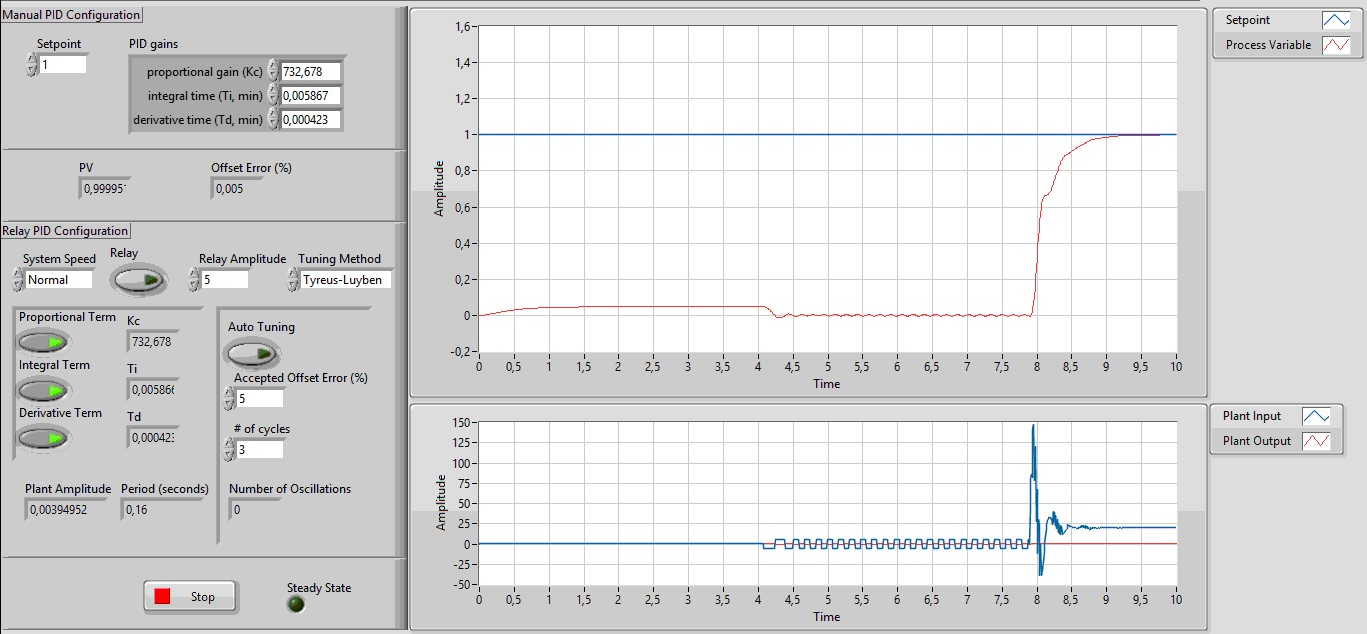
\includegraphics[width=\textwidth,height=5cm,keepaspectratio]{mass_springer_damper_TL}
  \caption{Βηματική απόκριση του συστήματος Μάζα-Ελατήριο-Αποσβεστήρας με εφαρμογή αναλογικού-ολοκληρωτικού-διαφορικού ελέγχου του οποίου τα κέρδη έχουν υπολογιστεί με τους τύπους Tyreus-Luyben}
  \label{fig:mass_springer_damper_TL}
\end{figure}



\subsubsection{Αντιμετώπιση Διαταραχών}
Στο Σχήμα \ref{fig:mass_spring_damper_disturbances} φαίνεται πώς το σύστημα αντιδράει στην ύπαρξη διαταραχών. Περίπου στο δέκατο τρίτο δευτερόλεπτο, γίνεται μια γρήγορη μεταβολή του setpoint η οποία ισοδυναμεί με μία σχεδόν στιγμιαία διαταραχή. Από το διάγραμμα της απόκρισης φαίνεται ότι το σύστημα έχει επανέλθει στην ηρεμία και έχει μηδενικό σφάλμα μόνιμης κατάστασης. 

\begin{figure}[h]
  \centering
  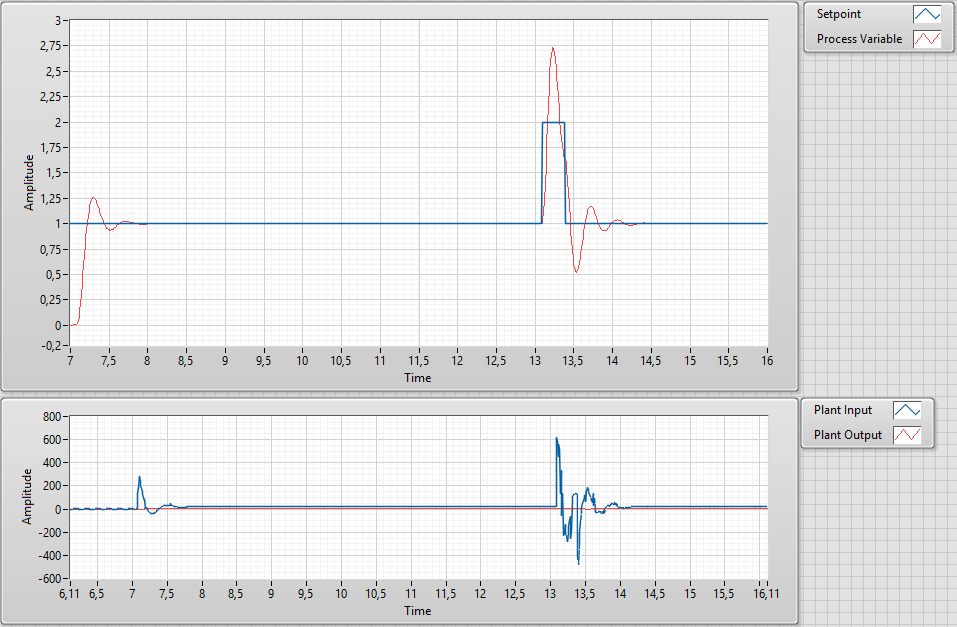
\includegraphics[width=\textwidth,height=5cm,keepaspectratio]{mass_spring_damper_disturbances}
  \caption{Αντιμετώπιση διαταραχών του αυτο-ρυθμιζόμενου PID ελεγκτή του οποίου τα κέρδη έχουν υπολογιστεί με τους τύπους Ziegler-Nichols}
  \label{fig:mass_spring_damper_disturbances}
\end{figure}

Όπως και πριν, έχει ενδιαφέρον να δούμε πώς διαχειρίζεται τις διαταραχές το σύστημα όταν τα κέρδη του ελεγκτή έχουν υπολογιστεί χρησιμοποιώντας διαφορετικούς τύπους. Έτσι, στο Σχήμα \ref{fig:mass_spring_damper_disturbances_slow} φαίνεται η προσπάθεια του ελεγκτή να ελέγξει το σύστημα σε διαταραχή, όταν τα κέρδη έχουν υπολογιστεί με τη μέθοδο Ziegler-Nichols και οι τύποι έχουν προσαρμοστεί για να δίνουν μια πιο αργή απόκριση.

\begin{figure}[h]
  \centering
  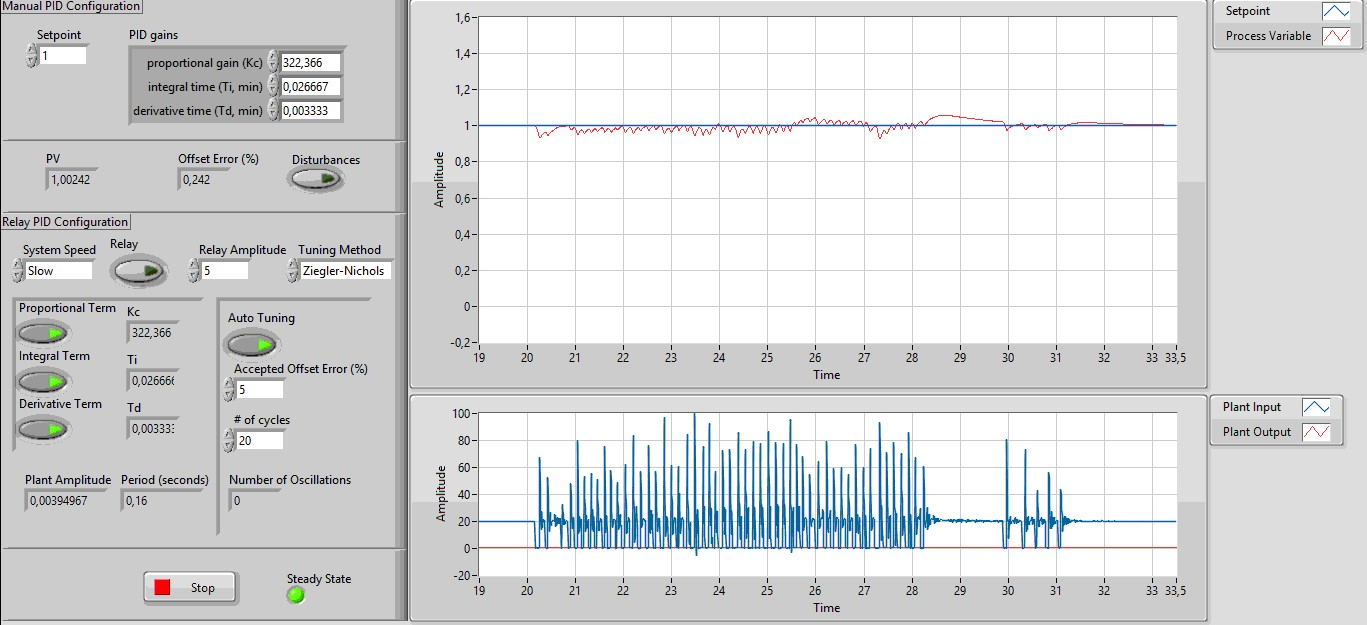
\includegraphics[width=\textwidth,height=5cm,keepaspectratio]{mass_spring_damper_disturbances_slow}
  \caption{Αντιμετώπιση διαταραχών του αυτο-ρυθμιζόμενου PID ελεγκτή του οποίου τα κέρδη έχουν υπολογιστεί με τους τύπους Ziegler-Nichols στη λειτουργία ``Slow"}
  \label{fig:mass_spring_damper_disturbances_slow}
\end{figure}

Τέλος, στο Σχήμα \ref{fig:mass_spring_damper_disturbances_TL} φαίνεται η αντιμετώπιση των διαταραχών όταν τα κέρδη έχουν υπολογιστεί με τους τύπους Tyreus-Luyben. Το σύστημα σταθεροποιείται πριν περάσει περισσότερο από ένα δευτερόλεπτο αλλά παρουσιάζει ένα μικρό ποσοστό υπέρβασης.

\begin{figure}[h]
  \centering
  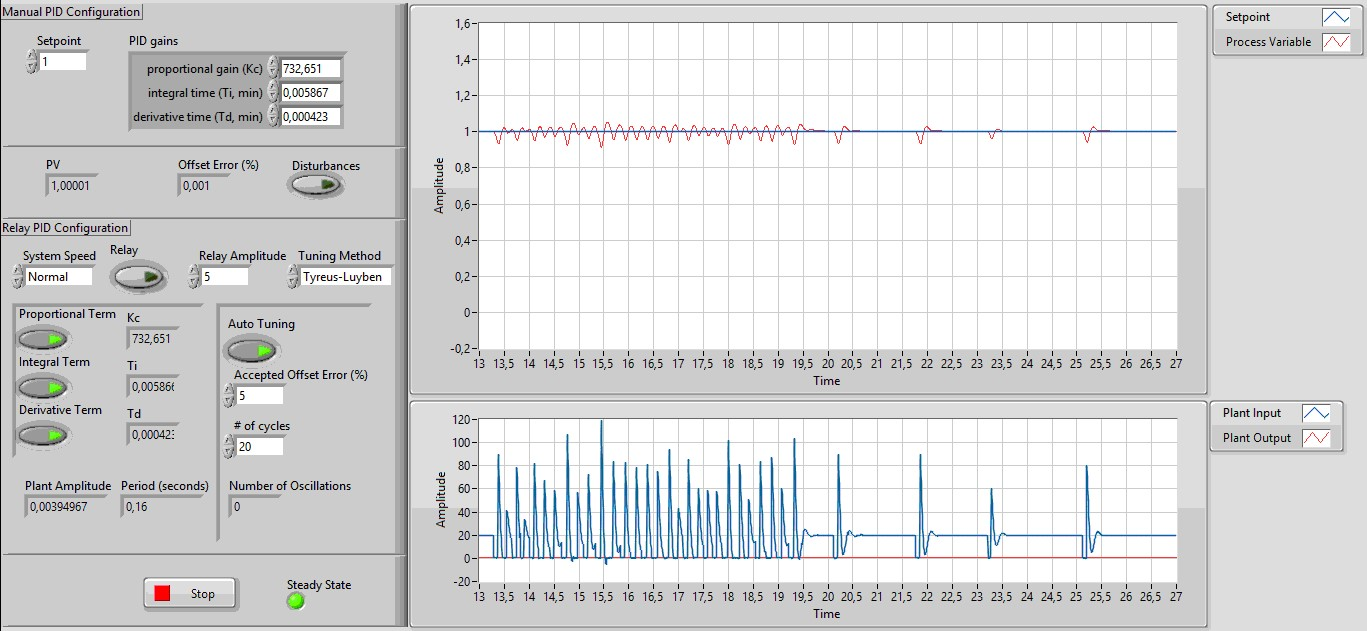
\includegraphics[width=\textwidth,height=5cm,keepaspectratio]{mass_spring_damper_disturbances_TL}
  \caption{Αντιμετώπιση διαταραχών του αυτο-ρυθμιζόμενου PID ελεγκτή του οποίου τα κέρδη έχουν υπολογιστεί με τους τύπους Tyreus-Luyben}
  \label{fig:mass_spring_damper_disturbances_TL}
\end{figure}

\subsection{Αποτελέσματα}

Στην ενότητα αυτή έγινε προσπάθεια να ελεγχθεί το κλασικό σύστημα ελέγχου που αποτελείται από μία μάζα, ένα ελατήριο και έναν αποσβεστήρα. Ως είσοδος του συστήματος θεωρήθηκε η δύναμη $F$ που ασκείται στη μάζα, ενώ ως έξοδος του συστήματος θεωρήθηκε η μετατόπιση $x$ που έχει η μάζα από το σημείο ισορροπίας της. 

Αρχικά, είδαμε ότι χωρίς έλεγχο το σύστημα δεν ανταποκρίνεται καλά καθώς έχει μεγάλο χρόνο ανύψωσης και μεγάλο σφάλμα μόνιμης κατάστασης. Έτσι στην αρχή χρησιμοποιήθηκε αναλογικός έλεγχος για τη μείωση του σφάλματος και τη βελτίωση του χρόνου ανύψωσης ο οποίος οδήγησε σε μία αξιοπρεπή απόκριση αλλά δεν κατάφερε να μηδενίσει το σφάλμα, παρά μόνο να το μειώσει σε ένα μικρό ποσοστό. 

Στη συνέχεια, χρησιμοποιήθηκε και ο ολοκληρωτικός όρος προκειμένου να μηδενιστεί το σφάλμα μόνιμης κατάστασης. Η τιμή του κέρδους όμως που υπολογίστηκε για τον ολοκληρωτικό όρο είχε σαν αποτέλεσμα να οδηγήσει το σύστημα σε μία μορφή αστάθειας. Αυτό οφείλεται στο ότι τόσο ο αναλογικός όσο και ο ολοκληρωτικός όρος μειώνουν το χρόνο ανύψωσης και ενισχύουν την υπερακόντιση του συστήματος οπότε προσθετικά οδηγούν την έξοδο του συστήματος σε ταλάντωση. Κανονικά, αν θα θέλαμε να έχουμε μόνο αναλογικό-ολοκληρωτικό έλεγχο θα έπρεπε, πριν την εφαρμογή του ολοκληρωτικού όρου, να μειώσουμε το αναλογικό κέρδος $K_c$. Όμως, στόχος μας στην παρούσα εργασία είναι να δούμε πόσο αποτελεσματικός είναι ο έλεγχος που παρέχει ο αυτο-ρυθμιζόμενος PID ελεγκτής που υλοποιήθηκε, χωρίς να πειράξουμε χειροκίνητα τα κέρδη που υπολογίζει.

Συνεπώς, για να βελτιώσουμε την απόκριση, προστέθηκε και ο διαφορικός όρος του ελεγκτή. Πλέον, ο έλεγχος που περιελάμβανε και τους τρεις όρους οδήγησε το σύστημα στο να έχει γρήγορο χρόνο ανύψωσης, μικρό ποσοστό υπερακόντισης και μηδενικό σφάλμα μόνιμης κατάστασης. Επίσης, αλλάζοντας την ταχύτητα που θέλουμε να έχει το κλειστό σύστημα ελέγχου ή επιλέγοντας τους τύπους Tyreus-Luyben αντί για τους Ziegler-Nichols, πετυχαίνουμε μια λιγότερο ``επιθετική" απόκριση. Παρόλο που είναι δύσκολο να πούμε ότι κάποιος έλεγχος είναι ξεκάθαρα καλύτερος από κάποιον άλλο αφού αυτό εξαρτάται από τις απαιτήσεις της κάθε διεργασίας, είναι ασφαλές να δηλώσουμε ότι τα κέρδη που υπολογίζονται με τους τύπους Tyreus-Luyben συνδυάζουν, ως ένα βαθμό, τις προηγούμενες αποκρίσεις, προσφέροντας έτσι τον περισσότερο ``σφαιρικό" έλεγχο.

\section{Σύστημα Cruise Control}

\subsection{Μαθηματικό Μοντέλο}

Το δεύτερο σύστημα που θα αναλυθεί είναι ένα πολύ καλό παράδειγμα ελέγχου ανάδρασης. Ο αυτόματος έλεγχος ταχύτητας ή \emph{cruise control} όπως είναι γνωστό στη διεθνή βιβλιογραφία, είναι ένα χαρακτηριστικό που βρίσκεται σε πολλά σύγχρονα αυτοκίνητα. Στόχος του είναι να κρατάει σταθερή την ταχύτητα του οχήματος, ανεξαρτήτως των διαταραχών που μπορεί να δέχεται από το περιβάλλον του, όπως η αντίσταση του ανέμου ή η κλίση του δρόμου. Αυτό το επιτυγχάνει μετρώντας την τρέχουσα ταχύτητα του οχήματος, συγκρίνοντας την με την επιθυμητή ταχύτητα και αυτόματα προσαρμόζοντας το γκάζι.

\begin{figure}[h]
  \centering
  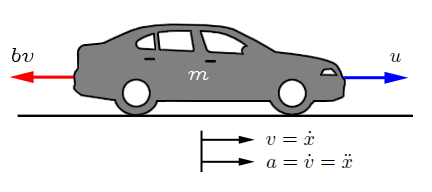
\includegraphics[width=\textwidth,height=5cm,keepaspectratio]{cruise_control_schematic}
  \caption{Μοντέλο συστήματος Αυτόματου Ελέγχου Ταχύτητας}
  \label{fig:cruise_control_schematic}
\end{figure}

Για την εύρεση των εξισώσεων του συστήματος, θεωρούμε ένα απλό μοντέλο της δυναμικής του οχήματος που φαίνεται στο παραπάνω διάγραμμα ελευθέρου σώματος. Το όχημα, μάζας $m$, ελέγχεται από μια δύναμη ελέγχου $u$. Η δύναμη αυτή αντιπροσωπεύει τη δύναμη που παράγεται στη διεπαφή δρόμου - ελαστικού. Για αυτό το απλοποιημένο μοντέλο, θα υποθέσουμε ότι μπορούμε να ελέγξουμε άμεσα αυτή τη δύναμη και θα παραμελήσουμε τη δυναμική του κινητήρα, των ελαστικών καθώς και των απωλειών που πηγαίνουν στη δημιουργία της δύναμης. Οι δυνάμεις αντίστασης, που οφείλονται στις τριβές των ελαστικών με το δρόμο και την αντίσταση του ανέμου, θεωρούμε ότι μεταβάλλονται γραμμικά με την ταχύτητα του οχήματος, $v$, και ενεργούν προς την αντίθετη κατεύθυνση από αυτή που κινείται το όχημα.

Με αυτές τις υποθέσεις, οδηγούμαστε σε ένα απλό σύστημα πρώτης τάξης. Αθροίζοντας τις δυνάμεις στον άξονα $x$ και εφαρμόζοντας τον $2^o$ Νόμο του Νεύτωνα, καταλήγουμε στην παρακάτω εξίσωση
\begin{equation}
m\dot{\upsilon} + b\upsilon = u
\label{eq:cruise_control_ode}
\end{equation}
όπου $u$ είναι η δύναμη που εφαρμόζεται στο όχημα και αποτελεί την είσοδο του συστήματος και $\upsilon$ είναι η ταχύτητα του οχήματος και αποτελεί την έξοδό του.

Παίρνοντας λοιπόν το μετασχηματισμό Laplace και στα δύο μέλη της εξίσωσης \ref{eq:cruise_control_ode} και θεωρώντας μηδενικές αρχικές συνθήκες, καταλήγουμε στη συνάρτηση μεταφοράς του συστήματος
\begin{equation}
P(s) = \frac{V(s)}{U(s)} = \frac{1}{ms+b} \left[\frac{m/s}{N}\right]
\label{eq:cruise_control_laplace}
\end{equation}

\subsection{Πείραμα}

Θεωρούμε ότι οι τιμές των παραμέτρων είναι $m = 1000\ kg$ και $\displaystyle b = 50\ \frac{Ns}{m}$. Με αντικατάσταση των τιμών στη συνάρτηση μεταφοράς έχουμε
\begin{equation}
\frac{V(s)}{U(s)} = \frac{1}{1000s+50}
\end{equation}

\subsubsection{Απόκριση Χωρίς Έλεγχο}

Αρχικά, ελέγχουμε να δούμε κατά πόσο το σύστημα χρειάζεται έλεγχο για να έχει ικανοποιητική απόδοση. Η απόκριση του συστήματος σε μια είσοδο βαθμίδας μοναδιαίου πλάτους φαίνεται στο παρακάτω σχήμα.

\begin{figure}[h]
  \centering
  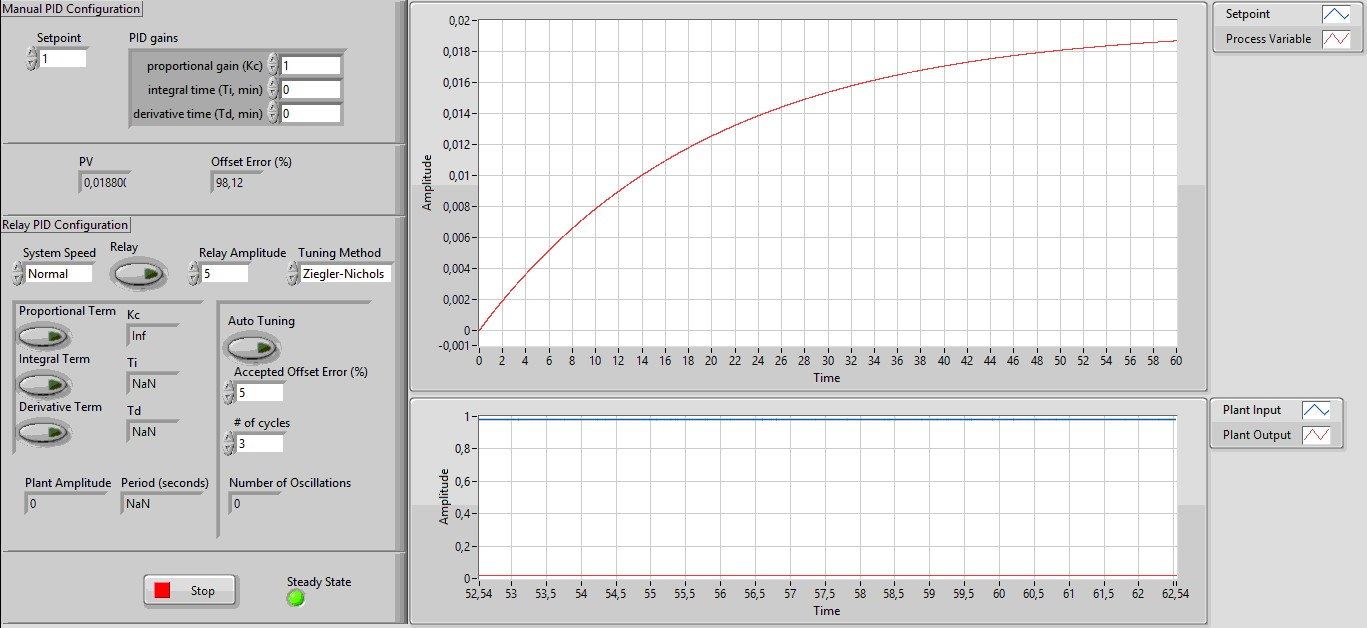
\includegraphics[width=\textwidth,height=5cm,keepaspectratio]{cruise_control_no_control}
  \caption{Βηματική απόκριση του συστήματος Αυτόματου Ελέγχου Ταχύτητας}
  \label{fig:cruise_control_no_control}
\end{figure}

Από την γραφική παράσταση βλέπουμε ότι η απόκριση του συστήματος χωρίς έλεγχο είναι πολύ αργή και έχει πολύ μεγάλο σφάλμα μόνιμης κατάστασης. 

%\subsubsection{Ταλαντώσεις του συστήματος}
%
%Επειδή το συγκεκριμένο σύστημα είναι πρώτης τάξεως, οι ταλαντώσεις που εκτελεί κατά το πείραμα relay, έχουν πολύ μικρό πλάτος και μικρή περίοδο. Το Σχήμα \ref{fig:cruise_control_oscillations} είναι η μεγέθυνση της απόκρισης του συστήματος έτσι ώστε να φανεί το πλάτος και η περίοδος των ταλαντώσεων αυτών. 
%
%\begin{figure}[h]
%  \centering
%  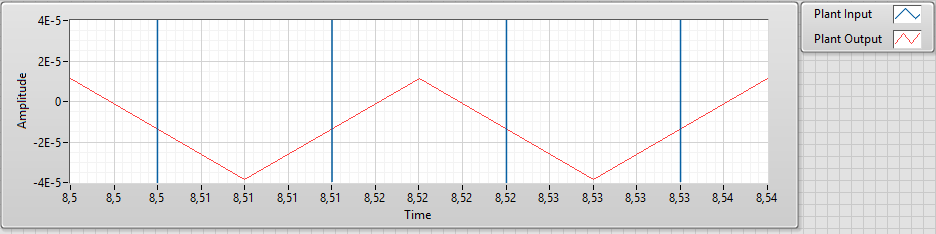
\includegraphics[width=\textwidth,height=5cm,keepaspectratio]{cruise_control_oscillations}
%  \caption{Ταλαντώσεις του συστήματος Αυτομάτου Ελέγχου Ταχύτητας}
%  \label{fig:cruise_control_oscillations}
%\end{figure}

\subsubsection{Αναλογικός Έλεγχος}

Στο Σχήμα \ref{fig:cruise_control_proportional} φαίνεται η απόκριση του συστήματος όταν ο PID ελεγκτής χρησιμοποιεί μόνο τον αναλογικό του όρο. Βλέπουμε ότι για το κέρδος του αναλογικού όρου έχει υπολογιστεί μια υπερβολικά μεγάλη τιμή, συγκεκριμένα $K_c = 176463$. Πέρα από αυτό, η απόκριση του συστήματος πλέον έχει βελτιωθεί καθώς φτάνει στο επιθυμητό σημείο σε περίπου έξι δευτερόλεπτα και το σφάλμα μόνιμης κατάστασης έχει πλέον τιμή $0.028\%$.

\begin{figure}[h]
  \centering
  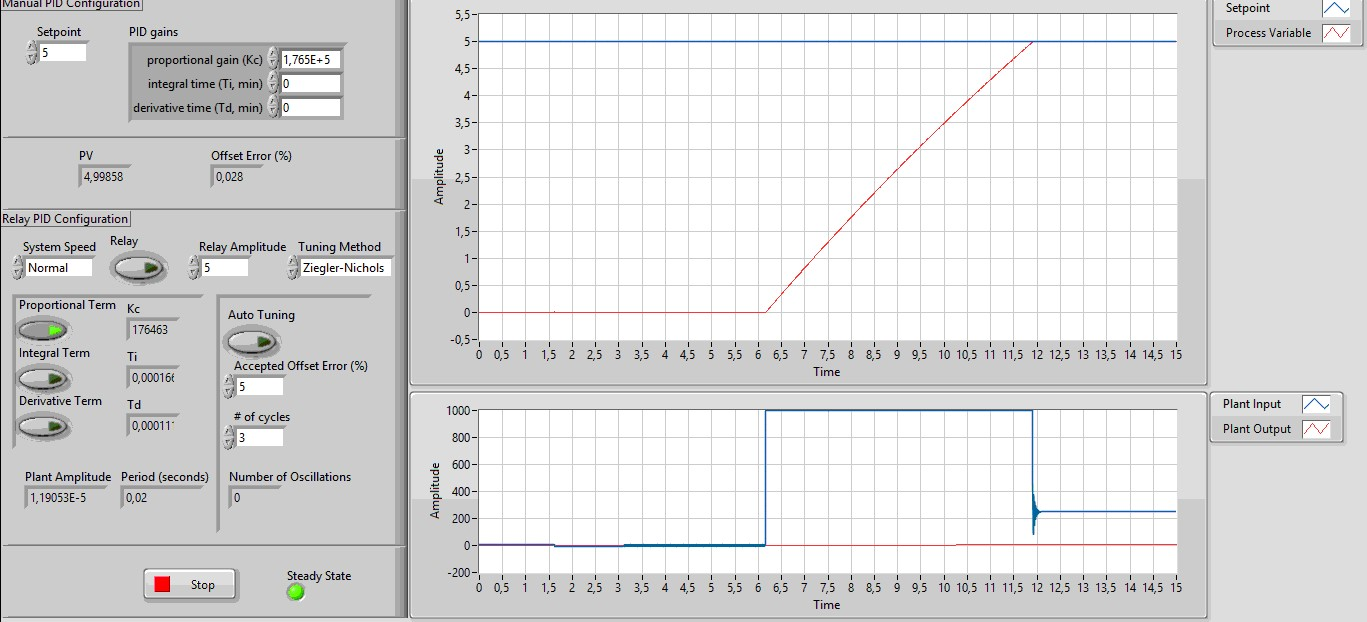
\includegraphics[width=\textwidth,height=5cm,keepaspectratio]{cruise_control_proportional}
  \caption{Βηματική απόκριση του συστήματος Αυτομάτου Ελέγχου Ταχύτητας με χρήση μόνο του αναλογικού όρου}
  \label{fig:cruise_control_proportional}
\end{figure}

\subsubsection{Αναλογικός - Ολοκληρωτικός Έλεγχος}

Στο Σχήμα \ref{fig:cruise_control_integral} φαίνεται η βηματική απόκριση του συστήματος όταν στον έλεγχο προστεθεί και ο ολοκληρωτικός όρος. Τόσο αυτή η απόκριση όσο και η προηγούμενη παρουσιάζουν πολλές ομοιότητες. Ο χρόνος ανύψωσης είναι σχεδόν ίδιος και η έξοδος του συστήματος έχει γραμμική μεταβολή συναρτήσει του χρόνου. Το μόνο που διαφέρει σε σχέση με πριν είναι ότι πλέον, λόγω του ολοκληρωτικού όρου, το σφάλμα μόνιμης κατάστασης είναι εντελώς μηδέν.

\begin{figure}[h]
  \centering
  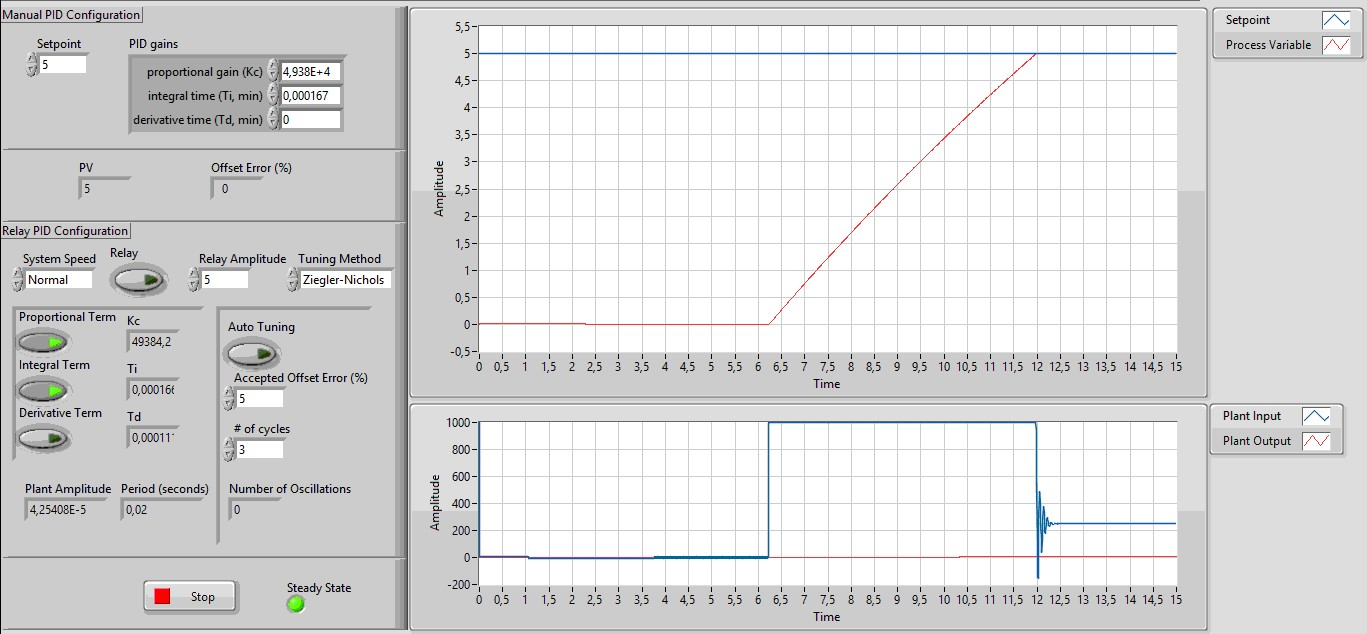
\includegraphics[width=\textwidth,height=5cm,keepaspectratio]{cruise_control_integral}
  \caption{Βηματική απόκριση του συστήματος Αυτομάτου Ελέγχου Ταχύτητας με χρήση του αναλογικού και του ολοκληρωτικού όρου}
  \label{fig:cruise_control_integral}
\end{figure}

\subsubsection{Αναλογικός - Ολοκληρωτικός - Διαφορικός Έλεγχος}

Στο Σχήμα \ref{fig:cruise_control_derivative} φαίνεται η απόκριση του συστήματος όταν ο ελεγκτής χρησιμοποιεί και τους τρεις όρους του. Από τη γραφική παράσταση εύκολα βγαίνει το συμπέρασμα ότι η απόκριση δεν άλλαξε καθόλου με την προσθήκη του διαφορικού όρου.

\begin{figure}[h]
  \centering
  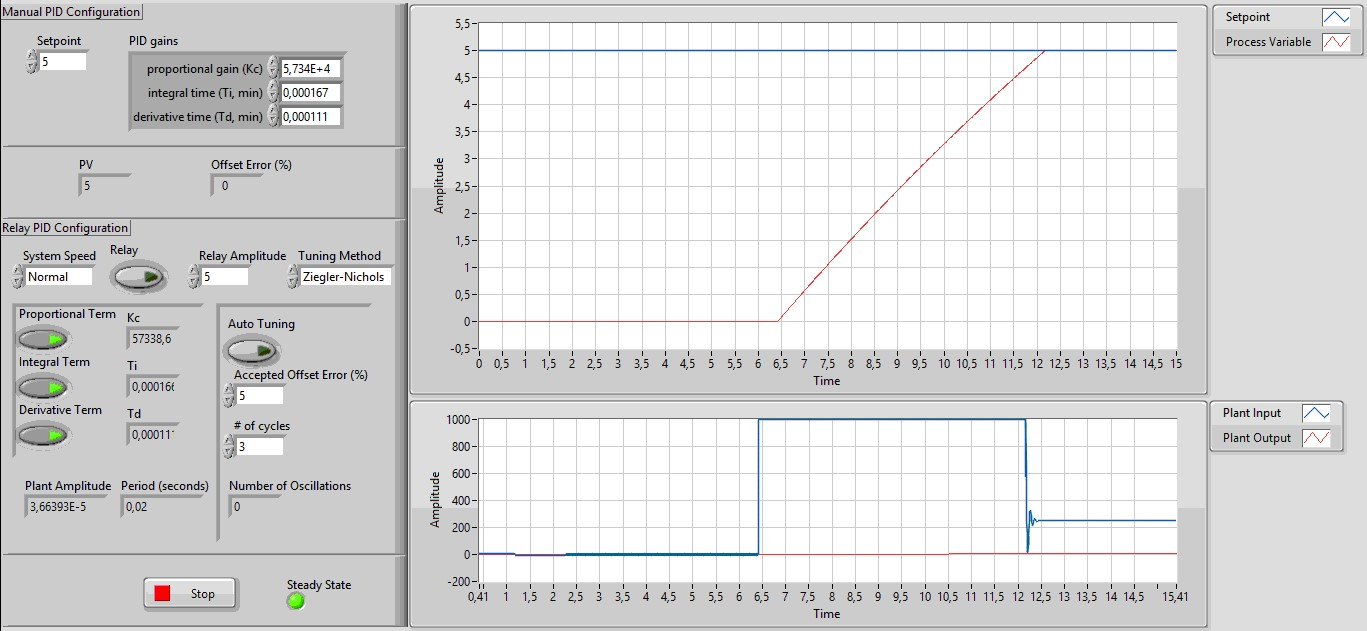
\includegraphics[width=\textwidth,height=5cm,keepaspectratio]{cruise_control_derivative}
  \caption{Βηματική απόκριση του συστήματος Αυτομάτου Ελέγχου Ταχύτητας με χρήση και των τριών όρων του PID ελεγκτή}
  \label{fig:cruise_control_derivative}
\end{figure}

Τέλος, στο Σχήμα \ref{fig:cruise_control_TL} φαίνεται η απόκριση του συστήματος όταν για τον αυτόματο υπολογισμό των κερδών του αναλογικού και του ολοκληρωτικού όρου έχουν χρησιμοποιηθεί οι τύποι Tyreus-Luyben. Όπως ήταν αναμενόμενο, ούτε σε αυτή την περίπτωση η απόκριση του συστήματος παρουσιάζει αλλαγές σε σχέση με τις προηγούμενες γραφικές παραστάσεις.

\begin{figure}[h]
  \centering
  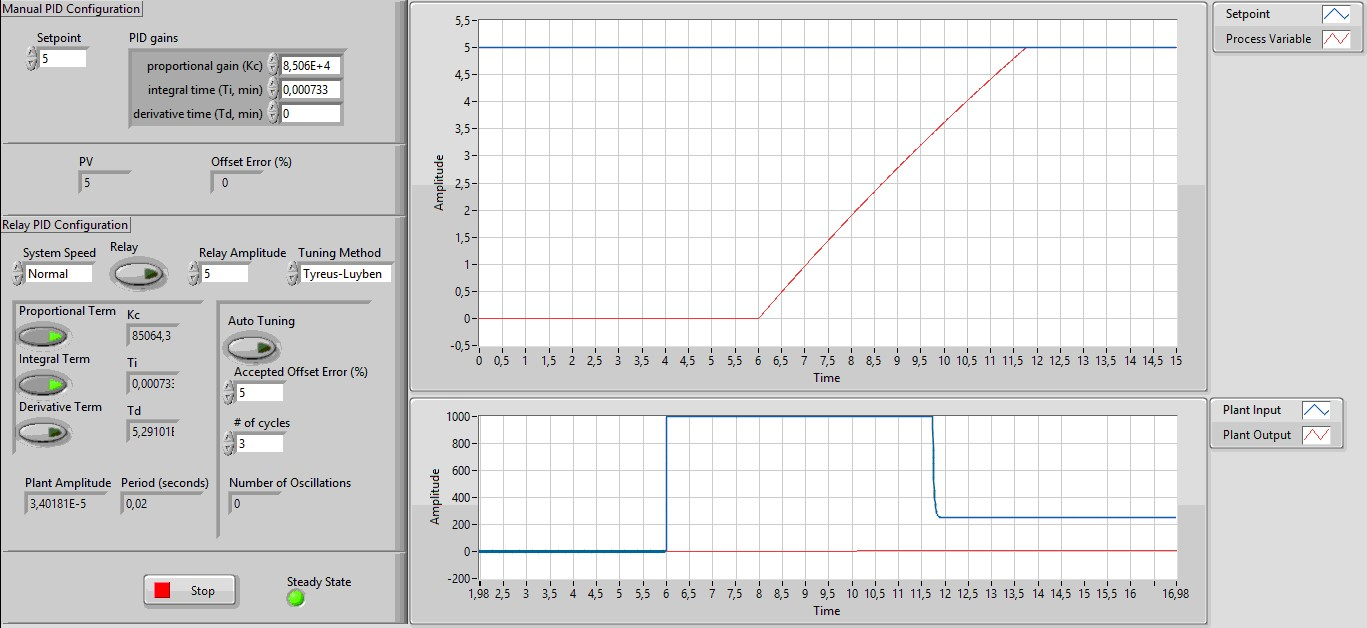
\includegraphics[width=\textwidth,height=5cm,keepaspectratio]{cruise_control_TL}
  \caption{Βηματική απόκριση του συστήματος Αυτομάτου Ελέγχου Ταχύτητας με χρήση και των τριών όρων του PID ελεγκτή όπου τα κέρδη έχουν υπολογιστεί χρησιμοποιώντας τους τύπους Tyreus-Luyben}
  \label{fig:cruise_control_TL}
\end{figure}

\subsubsection{Αντιμετώπιση Διαταραχών}

Αφού από τα διαδοχικά πειράματα καταλήξαμε στο συμπέρασμα ότι οι αποκρίσεις δεν έχουν αλλαγές μεταξύ τους, ο πιο ικανοποιητικός έλεγχος θα μπορούσαμε να πούμε ότι είναι αυτός που δεν περιλαμβάνει το διαφορικό όρο, αφού δεν προσφέρει κάτι παραπάνω. Στα σχήματα \ref{fig:cruise_control_disturbances} και \ref{fig:cruise_control_disturbances_TL} φαίνεται πώς το κλειστό σύστημα αποκρίνεται στις ξαφνικές διαταραχές που εισέρχονται στο βρόχο ελέγχου. Και σε αυτή την περίπτωση, οι δύο γραφικές παραστάσεις μοιάζουν υπερβολικά πολύ. Παρόλα αυτά, οι διαταραχές αντιμετωπίζονται ικανοποιητικά και το σύστημα επιστρέφει στην επιθυμητή τιμή μετά το πέρας αυτών. 

\begin{figure}[h]
  \centering
  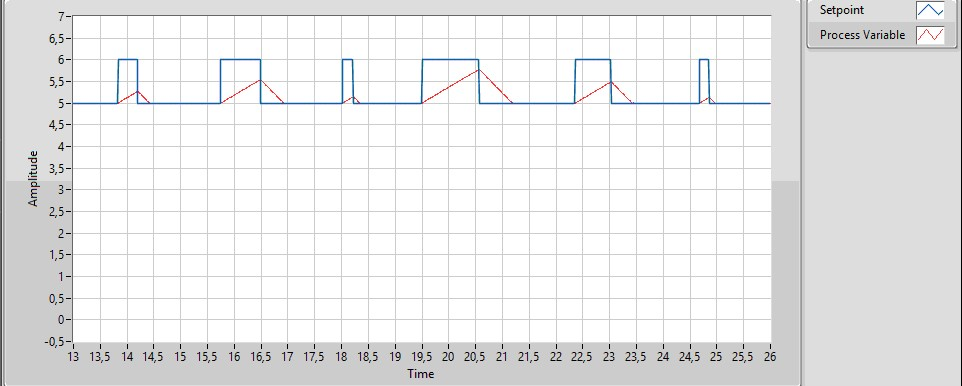
\includegraphics[width=\textwidth,height=5cm,keepaspectratio]{cruise_control_disturbances}
  \caption{Αντιμετώπιση διαταραχών του αυτο-ρυθμιζόμενου PID ελεγκτή του οποίου τα κέρδη έχουν υπολογιστεί με τους τύπους Ziegler-Nichols}
  \label{fig:cruise_control_disturbances}
\end{figure}

\begin{figure}[h]
  \centering
  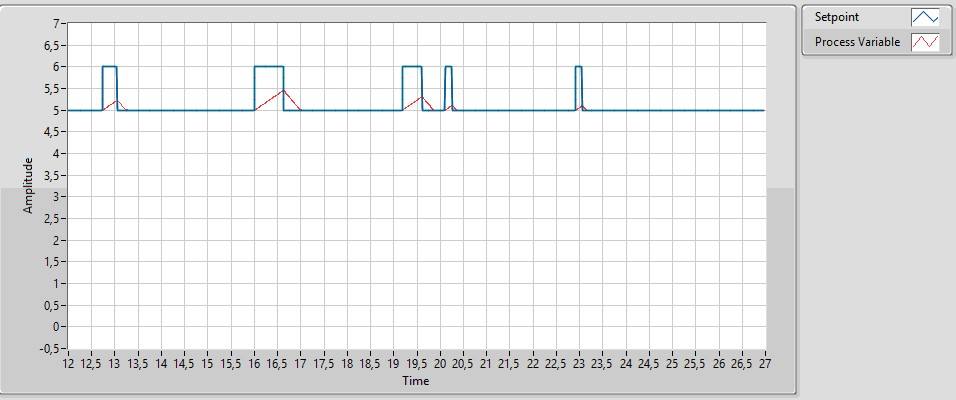
\includegraphics[width=\textwidth,height=5cm,keepaspectratio]{cruise_control_disturbances_TL}
  \caption{Αντιμετώπιση διαταραχών του αυτο-ρυθμιζόμενου PID ελεγκτή του οποίου τα κέρδη έχουν υπολογιστεί με τους τύπους Tyreus-Luyben}
  \label{fig:cruise_control_disturbances_TL}
\end{figure}

\subsection{Αποτελέσματα}

Σε αυτή την ενότητα έγινε προσπάθεια να ελεγχθεί ένα σύστημα που συναντάται σε καθημερινή βάση σε όλα τα σύγχρονα οχήματα. Αρχικά, με μία απλή προσομοίωση κατέστη εμφανές ότι το σύστημα χρήζει ελέγχου, αφού χωρίς ελεγκτή η απόκριση ήταν πολύ αργή και η τελική τιμή της εξόδου του συστήματος ήταν περίπου $0.02$ αντί για $1$ που ήταν το επιθυμητό. Αυτό είναι λογικό αφού η συνάρτηση μεταφοράς (Εξίσωση \ref{eq:cruise_control_laplace}) για τις δοθείσες τιμές των παραμέτρων έχει κέρδος ανοιχτού βρόχου $\displaystyle \frac{1}{50} = 0.02$.

Προχωρώντας λοιπόν στον έλεγχο του συστήματος παρατηρήθηκε κάτι αρκετά ενδιαφέρον. Ασχέτως με τον τύπο ελέγχου που χρησιμοποιήθηκε ή τη μέθοδο με την οποία υπολογίστηκαν τα κέρδη, η απόκριση του κλειστού συστήματος φαίνεται να μένει ανεπηρέαστη.  































































